\documentclass{article}
\usepackage{tkz-graph}
\usepackage{paralist}
\pagestyle{empty}
\usetikzlibrary{patterns}

\begin{document}

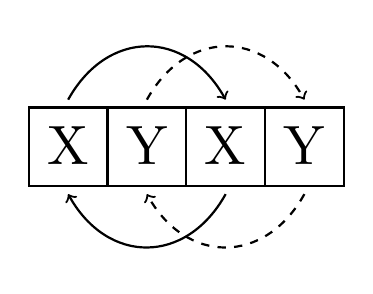
\begin{tikzpicture}

\draw[thick] (0,0) rectangle (1,1);
\draw[thick] (1,0) rectangle (2,1);
\draw[thick] (2,0) rectangle (3,1);
\draw[thick] (3,0) rectangle (4,1);

\draw (0.5,1) node[anchor=north, scale=2] {X};
\draw (1.5,1) node[anchor=north, scale=2] {Y};
\draw (2.5,1) node[anchor=north, scale=2] {X};
\draw (3.5,1) node[anchor=north, scale=2] {Y};

\draw[thick,->] (0.5,1.1) .. controls (1,2) and (2,2) .. (2.5,1.1);
\draw[dashed,thick,->] (1.5,1.1) .. controls (2,2) and (3,2) .. (3.5,1.1);
\draw[dashed,thick,->] (3.5,-0.1) .. controls (3,-1) and (2,-1) .. (1.5,-0.1);
\draw[thick,->] (2.5,-0.1) .. controls (2,-1) and (1,-1) .. (0.5,-0.1);

\end{tikzpicture}

\end{document}